
\documentclass[twoside]{article}

\usepackage{graphicx}% Include figure files
\usepackage{dcolumn}% Align table columns on decimal point
\usepackage{bm}% bold math
\usepackage{hyperref}% add hypertext capabilities
\setlength{\marginparwidth}{2cm}
\usepackage{comment}

%\usepackage[hidelinks]{hyperref}% add hypertext capabilities

%\usepackage[mathlines]{lineno}% Enable numbering of text and display math
%\linenumbers\relax % Commence numbering lines


\hypersetup{
    %bookmarks=true,         % show bookmarks bar? % Already true
    unicode=false,          % non-Latin characters
    pdftoolbar=true,        % show Acrobat
    pdfmenubar=true,        % show Acrobat
    pdffitwindow=false,     % window fit to page when opened
    pdfstartview={FitH},    % fits the width of the page to the window
    pdftitle={Transverse-electric surface plasmon polaritons in periodically modulated graphene},    % title
    pdfauthor={Ahmad, Oh, Muljarov},     % author
    pdfsubject={},   % subject of the document
    pdfcreator={},   % creator of the document
    pdfproducer={}, % producer of the document
    pdfkeywords={} {} {}, % list of keywords
    pdfnewwindow=true,      % links in new window
    colorlinks=true,       % false: boxed links; true: colored links
    linkcolor=blue, %red,          % color of internal links (change box color with linkbordercolor)
    citecolor=blue,        % color of links to bibliography
    filecolor=magenta,      % color of file links
    urlcolor=blue,           % color of external links
	breaklinks=true
}


\begin{document}



\title{Example title of paper}

\author{Joe Author}

\author{Another Author}
\author{Another one}

\date{\today}
\begin{abstract}
This paper is for demonstrating how figurer can work
\end{abstract}

\maketitle

\section{\label{sec:level1}Introduction}

This is introduction.

\begin{figure}[]
\centering
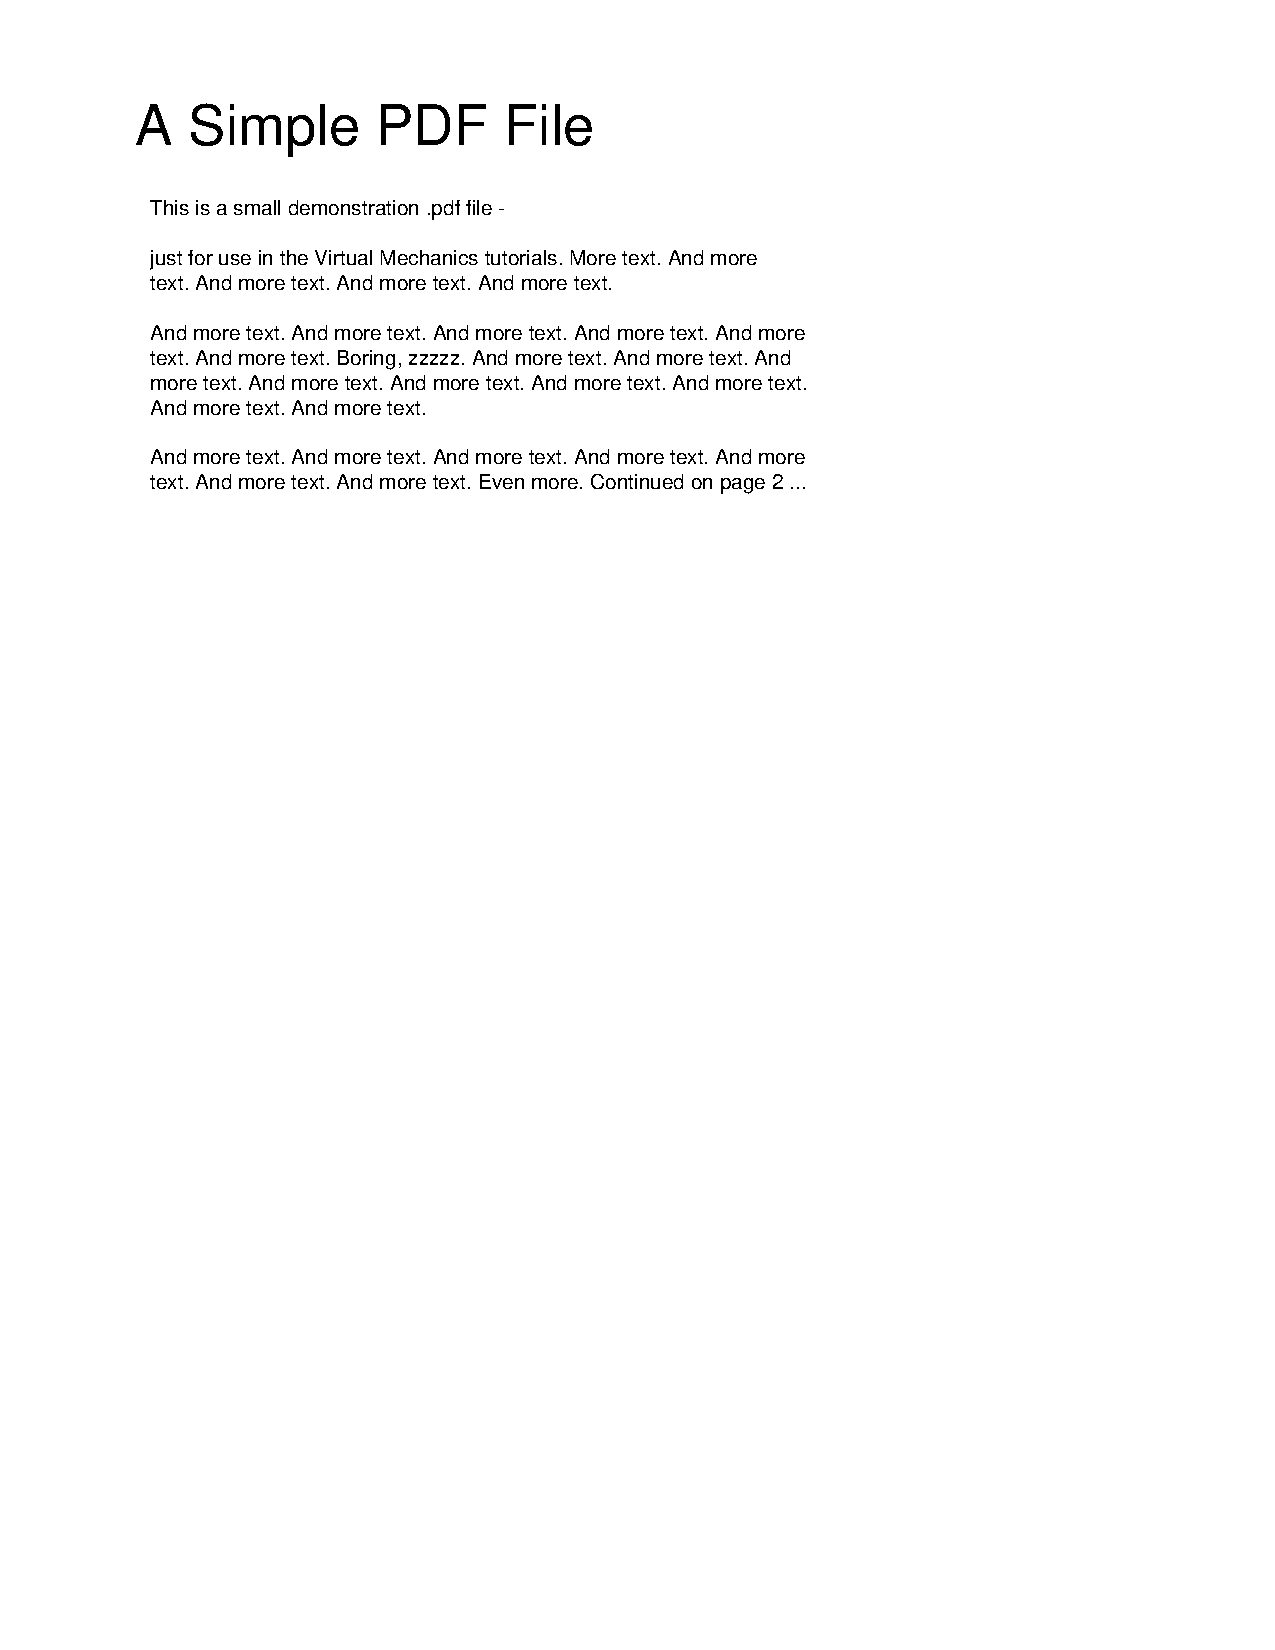
\includegraphics[]{examplefiga.pdf}
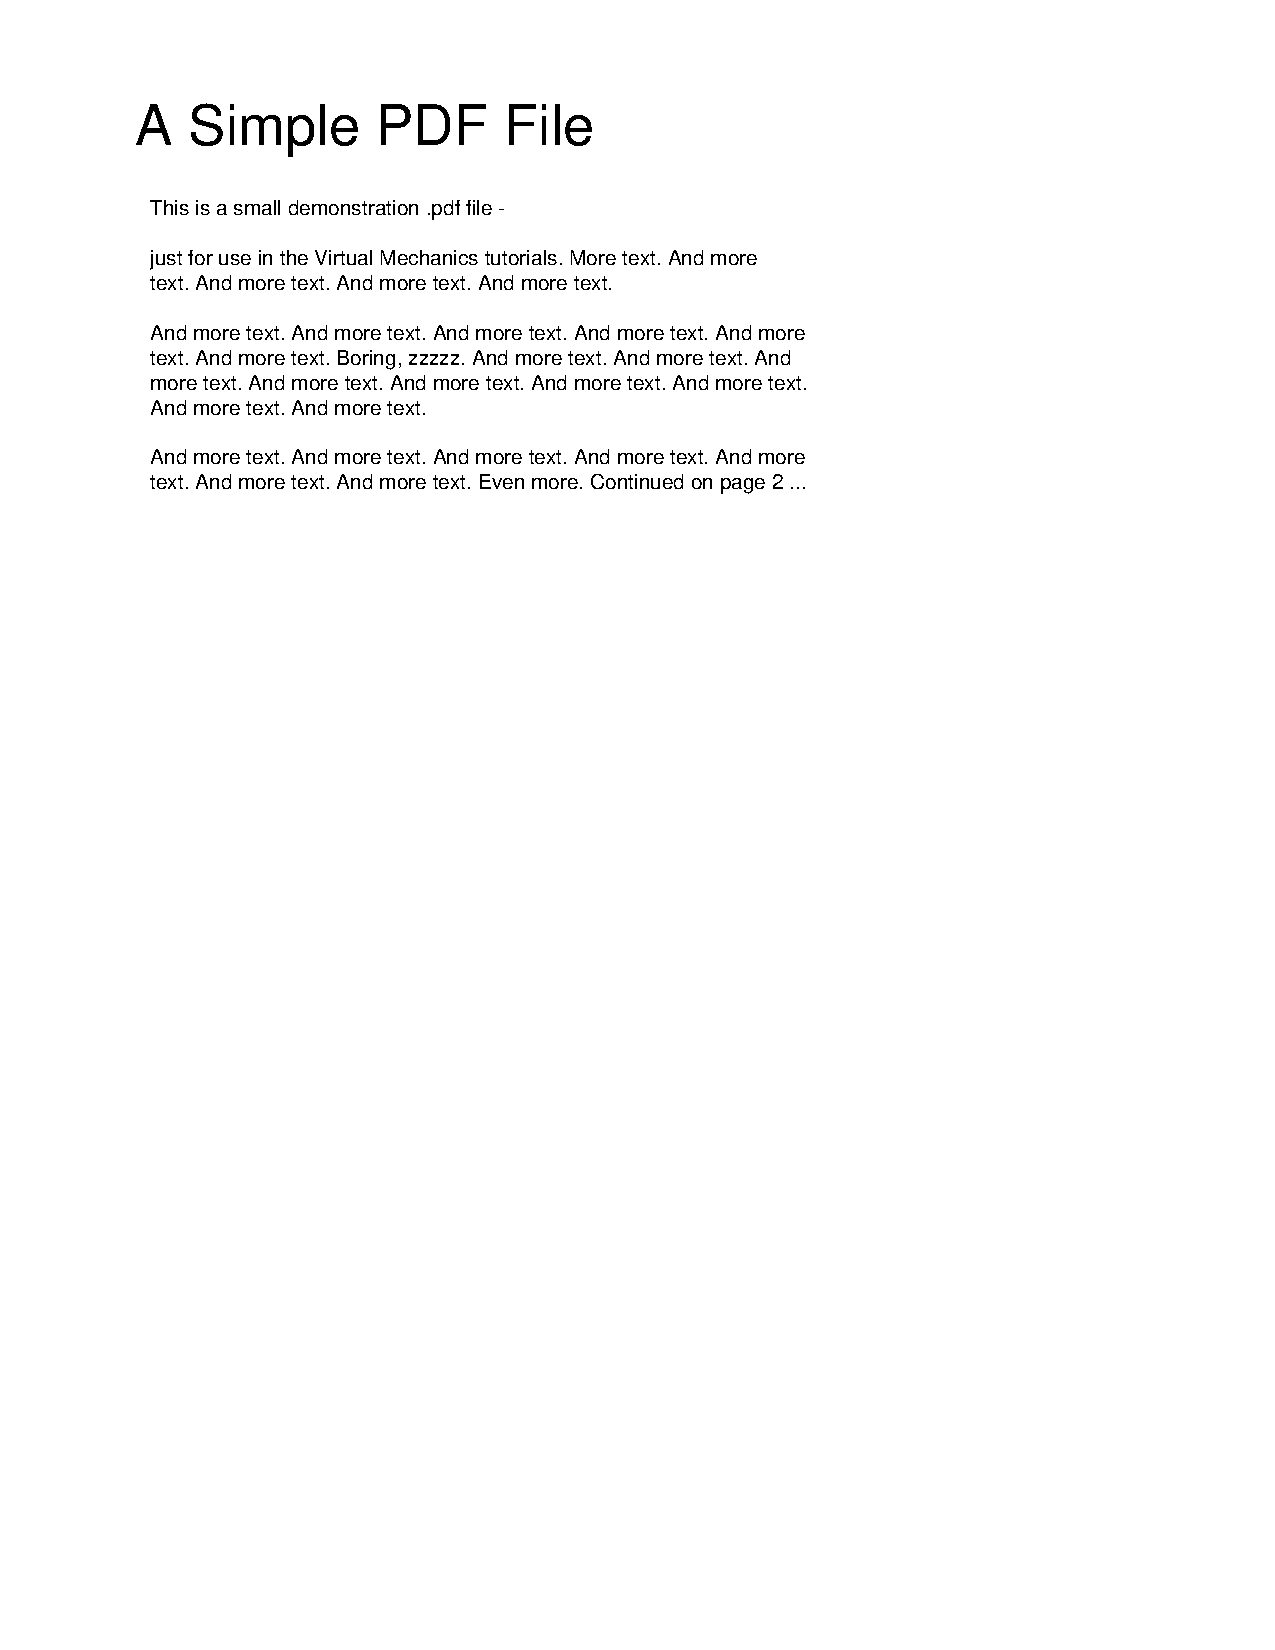
\includegraphics[]{examplefigb.pdf}
\caption{This is an example of a latex figure containing two figurer figures. Okay it is confusing.}
\label{example_fig}
\end{figure}

\section{Model}

In this section, we write stuff about the model.

\section{Conclusions}
\label{Sec:summary}
We finally conclude the paper.

\section*{Acknowledgments}
Make some acknowledgements.

\appendix


\section{The title of appendix} \label{appendix1}
%-----------------------------------------------------------------------------
This is an appendix

\end{document}





